\documentclass[]{article}
\usepackage{graphicx}
\usepackage[svgnames]{xcolor} 
\usepackage{fancyhdr}
\usepackage{fancyvrb}
\usepackage{forest}
\usepackage{tocloft}
\usepackage[hidelinks]{hyperref}
\usepackage{enumitem}
\usepackage[many]{tcolorbox}
\usepackage{listings }
\usepackage[a4paper, total={6in, 8in} , top = 2cm,bottom = 4cm]{geometry}
%\usepackage[a4paper, total={6in, 8in}]{geometry}
\usepackage{afterpage}
\usepackage{amssymb}
\usepackage{pdflscape}
\usepackage{textcomp}
\usepackage{xecolor}
\usepackage{rotating}
\usepackage[Kashida=on,KashidaXBFix=on]{xepersian}
\usepackage[T1]{fontenc}
\usepackage{tikz}
\usepackage[utf8]{inputenc}
\usepackage{PTSerif} 
\usepackage{seqsplit}
\usepackage{changepage}


\usepackage{listings}
\usepackage{xcolor}
\usepackage{sectsty}

\setcounter{secnumdepth}{0}
 
\definecolor{codegreen}{rgb}{0,0.6,0}
\definecolor{codegray}{rgb}{0.5,0.5,0.5}
\definecolor{codepurple}{rgb}{0.58,0,0.82}
\definecolor{backcolour}{rgb}{0.95,0.95,0.92}
\definecolor{blanchedalmond}{rgb}{1.0, 0.92, 0.8}
\definecolor{brilliantlavender}{rgb}{0.96, 0.73, 1.0}
 
\NewDocumentCommand{\codeword}{v}{
\texttt{\textcolor{blue}{#1}}
}
\lstset{language=java,keywordstyle={\bfseries \color{blue}}}

\lstdefinestyle{mystyle}{
    backgroundcolor=\color{backcolour},   
    commentstyle=\color{codegreen},
    keywordstyle=\color{magenta},
    numberstyle=\tiny\color{codegray},
    stringstyle=\color{codepurple},
    basicstyle=\ttfamily\normalsize,
    breakatwhitespace=false,         
    breaklines=true,                 
    captionpos=b,                    
    keepspaces=true,                 
    numbers=left,                    
    numbersep=5pt,                  
    showspaces=false,                
    showstringspaces=false,
    showtabs=false,                  
    tabsize=2
}

\lstset{style=mystyle}

 \settextfont[BoldFont={XB Zar bold.ttf}]{XB Zar.ttf}


\setlatintextfont[Scale=1.0,
 BoldFont={LiberationSerif-Bold.ttf}, 
 ItalicFont={LiberationSerif-Italic.ttf}]{LiberationSerif-Regular.ttf}





\newcommand{\inputsample}[1]{
    ~\\
    \textbf{ورودی نمونه}
    ~\\
    \begin{tcolorbox}[breakable,boxrule=0pt]
        \begin{latin}
            \large{
                #1
            }
        \end{latin}
    \end{tcolorbox}
}

\newcommand{\outputsample}[1]{
    ~\\
    \textbf{خروجی نمونه}

    \begin{tcolorbox}[breakable,boxrule=0pt]
        \begin{latin}
            \large{
                #1
            }
        \end{latin}
    \end{tcolorbox}
}

\newtcolorbox{mybox}[2][]{colback=red!5!white,
colframe=red!75!black,fonttitle=\bfseries,
colbacktitle=red!85!black,enhanced,
attach boxed title to top center={yshift=-2mm},
title=#2,#1}

\newenvironment{changemargin}[2]{%
\begin{list}{}{%
\setlength{\topsep}{0pt}%
\setlength{\leftmargin}{#1}%
\setlength{\rightmargin}{#2}%
\setlength{\listparindent}{\parindent}%
\setlength{\itemindent}{\parindent}%
\setlength{\parsep}{\parskip}%
}%
\item[]}{\end{list}}


\definecolor{foldercolor}{RGB}{124,166,198}
\definecolor{sectionColor}{HTML}{ff5e0e}
\definecolor{subsectionColor}{HTML}{008575}

\definecolor{listColor}{HTML}{00d3b9}

\definecolor{umlrelcolor}{HTML}{3c78d8}

\definecolor{subsubsectionColor}{HTML}{3c78d8}

\defpersianfont\authorFont[Scale=0.9]{XB Zar bold.ttf}

\defpersianfont\titr[Scale=1.5]{Lalezar-Regular.ttf}

\defpersianfont\fehrest[Scale=1.2]{Lalezar-Regular.ttf}

\defpersianfont\fehrestTitle[Scale=3.0]{Lalezar-Regular.ttf}

\defpersianfont\fehrestContent[Scale=1.2]{XB Zar bold.ttf}


\sectionfont{\color{sectionColor}}  % sets colour of sections
\subsectionfont{\color{subsectionColor}}  % sets colour of sections
\subsubsectionfont{\color{subsubsectionColor}}


\renewcommand{\labelitemii}{$\circ$}


\renewcommand{\baselinestretch}{1.1}


\renewcommand{\contentsname}{فهرست}

\renewcommand{\cfttoctitlefont}{\fehrestTitle}


\renewcommand\cftsecfont{\color{sectionColor}\fehrestContent\selectfont}
\renewcommand\cftsubsecfont{\color{subsectionColor}\fehrestContent\selectfont}
\renewcommand\cftsubsubsecfont{\color{subsubsectionColor}\fehrestContent\selectfont}
%\renewcommand{\cftsecpagefont}{\color{sectionColor}}

\setlength{\parskip}{1.2pt}

\begin{document}


%%% title pages
\begin{titlepage}
\begin{center}

\textbf{ \Huge{به نام خدا} }
        
\vspace{0.2cm}


\includegraphics[width=0.4\textwidth]{sharif1.png}\\
\vspace{0.2cm}
\textbf{ \Huge{\emph درس برنامه‌سازی پیشرفته} }\\
\vspace{0.25cm}
\textbf{ \Large{ آموزش کار با ابزار \lr{ngrok}} }
\vspace{0.2cm}
       
 
      \large \textbf{دانشکده مهندسی کامپیوتر}\\\vspace{0.1cm}
    \large   دانشگاه صنعتی شریف\\\vspace{0.2cm}
       \large   ﻧﯿﻢ سال دوم 00-99 \\\vspace{0.10cm}
      \noindent\rule[1ex]{\linewidth}{1pt}
استاد:\\
    \textbf{{دکتر محمدامین فضلی}}



    \vspace{0.10cm}
تهیه‌کننده محتوا:\\
    \textbf{\authorFont{امیرمهدی نامجو}}
    
\end{center}
\end{titlepage}
%%% title pages


%%% header of pages
\newpage
\pagestyle{fancy}
\fancyhf{}
\fancyfoot{}
\cfoot{\thepage}
\lhead{فاز سوم}
\rhead{
\includegraphics[width=0.1\textwidth]{sharif.png}\\
دانشکده مهندسی کامپیوتر
}
\chead{پروژه برنامه‌سازی پیشرفته}
%%% header of pages
\renewcommand{\headrulewidth}{2pt}

\KashidaOff



\newpage

 \Large \textbf{\\\\
}


\section*{{\titr چه نیازی به \lr{ngrok} داریم؟}}
\addcontentsline{toc}{section}{{\fehrestContent چه نیازی به \lr{ngrok} داریم؟}}

احتمالا تا به حال در طول تمرین و فاز سوم پروژه، کدهایی نوشته‌اید که با شبکه کار کنند و احتمالا تمامی این کدها را روی شبکه محلی کامپیوتر خود اجرا کرده‌اید. شاید برایتان سوال باشد که چگونه می‌توان پس از اجرای کد، از طریق یک کامپیوتر دیگر و بر بستر اینترنت به آن برنامه درخواست ارسال کرد؟

اگر سرور خریداری کرده باشید و یا اینرنت ثابتی که در اختیار دارید، آی‌پی ثابت (\lr{Static IP}) داشته باشد، می‌توانید به راحتی با بدست آوردن \lr{IP} آن از طریق گوگل از طریق سرچ کردن عبارت \lr{What is my IP} به راحتی از بیرون  از طریق آن \lr{IP} آدرس و پورت مشخصی که برنامه شما روی آن گوش می‌دهد، به آن دسترسی پیدا کنید.

با این وجود، عموما  \lr{ISP} هایی که اینترنت \lr{ADSL} ارائه می‌دهند، کاربران را پشت سیستمی به نام \lr{NAT} قرار می‌دهند. به طور خلاصه \lr{NAT} یا \lr{Network Address Translation} باعث می‌شود که تعداد سیستم مجزا، همگی یک آی‌پی یکسان از بیرون پیدا کنند. یعنی عملا شما درون شبکه \lr{NAT} یک آی‌پی خصوصی دارید که از بیرون قابل دسترس نیست و هر پیامی که می فرستید با عبور از \lr{NAT}، یک آی‌پی عمومی خاص که مربوط به آن \lr{NAT} می‌شود را پیدا کرده و از طریق آن پیام ارسال می‌شود. در نتیجه کاربران مختلفی که پشت \lr{NAT} هستند، همگی از طریق یک آی‌پی ارتباط برقرار می‌کنند.

در نتیجه این موضوع، سیستم‌های دیگر نمی‌توانند مستقیما شروع کننده ارتباط با سیستم شما باشند. در اصل همیشه سیستم شما شروع کننده ارتباط با بیرون است و پس از عبور پیام از \lr{NAT}، براساس آی‌پی و پورت مبدا و مقصد، \lr{NAT} متوجه می‌شود که جواب‌های بعدی که دریافت می‌شود را به کدام یک از کامپیوترهای شبکه درونی ارسال کند.

با توجه به این موضوع برای این که بتوانید از بیرون به کامپیوتر خود وصل شوید، نیازمند ابزارهای جانبی هستید. \lr{ngrok} یک ابزار رایگان است که این امکان را برای شما فراهم می‌کند. کارکرد \lr{ngrok} به این صورت است که شما ارتباط اولیه را با آن برقرار می‌کنید و با برقرار شدن این ارتباط، \lr{ngrok} می‌تواند به راحتی پیام‌ها را برای شما ارسال کند. حال \lr{ngrok} نقش یک واسط را ایفا کرده و افراد دیگری که قصد اتصال به شما را داشته باشند، می‌توانند درخواست خود را به \lr{ngrok} فرستاده و \lr{ngrok} با توجه به برقرار بودن ارتباط، درخواست آنان را برای شما ارسال می‌کند.

 


\newpage

\section*{{\titr نحوه کار با \lr{ngrok}}}
\addcontentsline{toc}{section}{{\fehrestContent نحوه کار با \lr{ngrok}}}

برای کار با \lr{ngrok} لازم است به سایت آن یعنی 
 \href{ngrok.com}{ngrok.com}
 بروید و با کلیک روی گزینه \lr{Sign Up} در سایت آن ثبت نام کنید. البته بدون ثبت نام هم می‌توان از آن استفاده کرد اما تنها پروتکل \lr{HTTP} در دسترس خواهد بود و از آن‌جایی که به احتمال زیاد پروژه شما از طریق پروتکل \lr{TCP} کار می‌کند، نیازمند ثبت نام در این سایت هستید.
 
 پس از ثبت نام با صفحه زیر رو به رو می‌شوید:
 
 \begin{center}
 	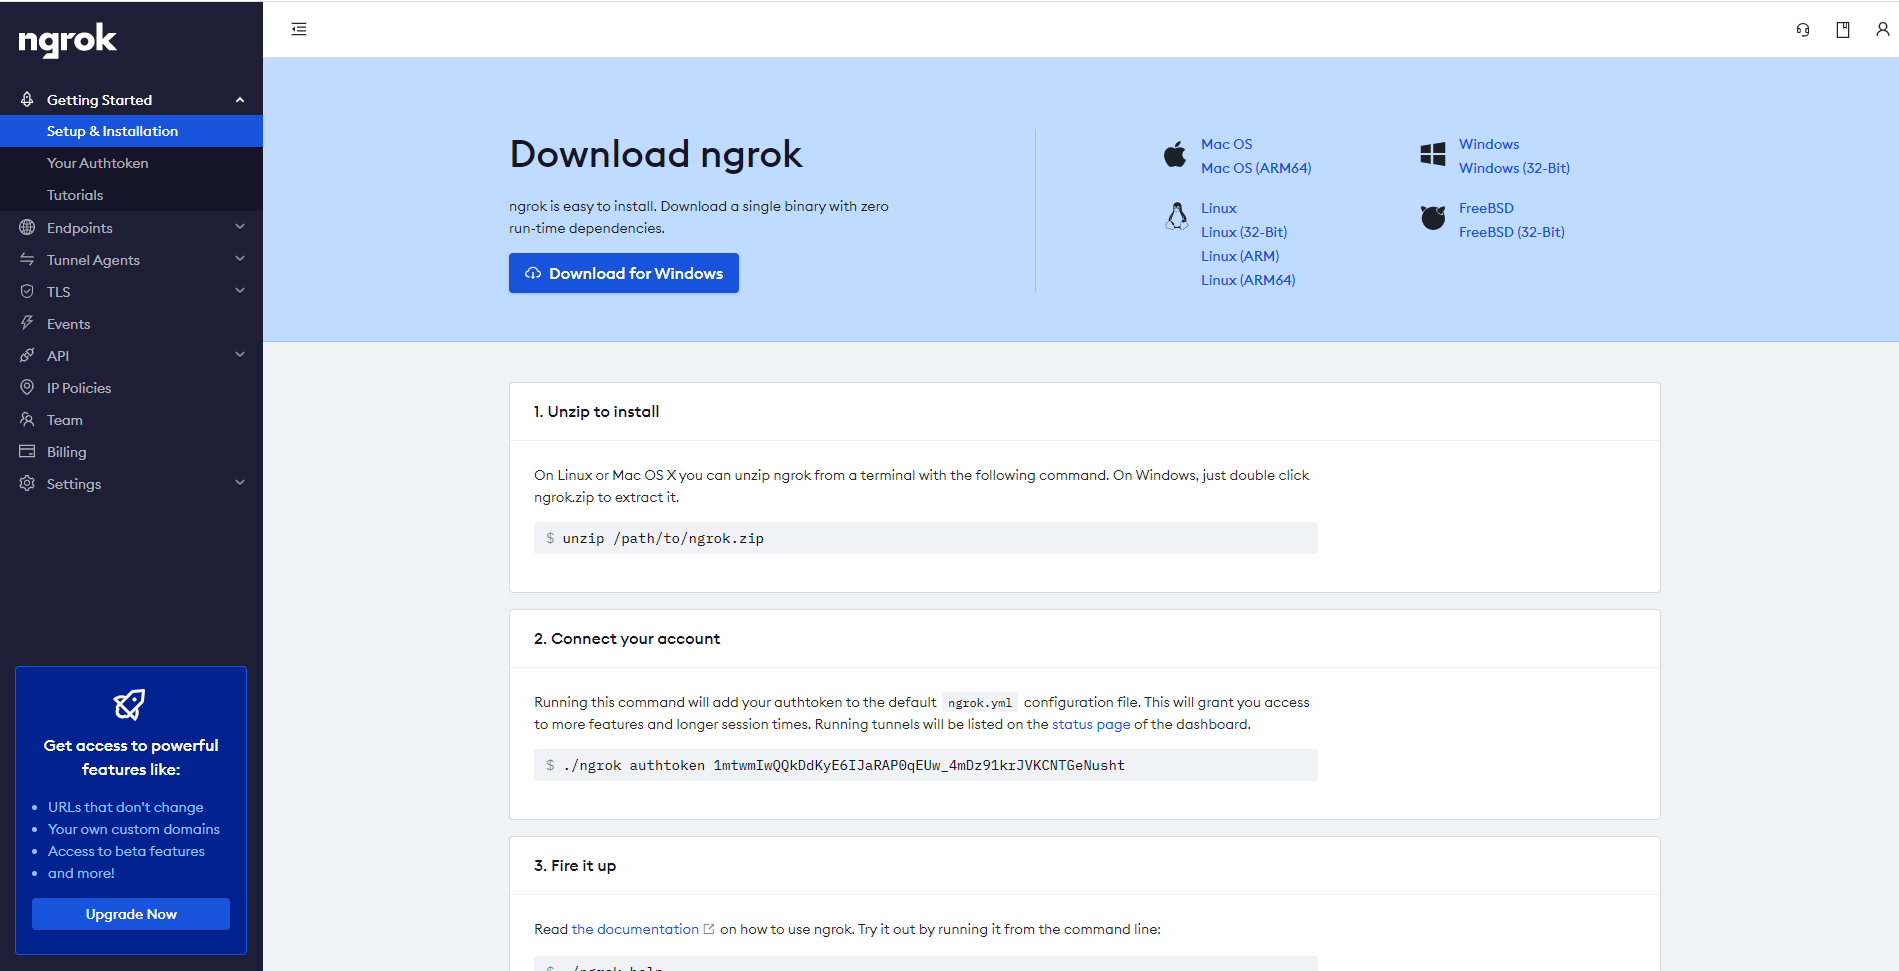
\includegraphics[width = 1.0 \textwidth]{images/1.png}
 \end{center}

در این صفحه متناسب با سیستم عامل خود، نسخه مربوط را دانلود کنید. پس از دانلود، با یک فایل فشرده رو به رو خواهید شد و پس از اکسترکت کردن آن، فایلی به نام \lr{ngrok} در اختیار دارید (در سیستم عامل ویندوز این فایل پسوند  \lr{.exe} هم دارد).

این فایل را در جایی اکسترکت کرده و سپس از طریق \lr{CMD} (در ویندوز) یا ترمینال (در MacOS یا لینوکس) به آن پوشه رفته و دستور زیر را اجرا کنید:
\begin{latin}
\begin{lstlisting}[language = bash]
./ngrok authtoken 1mtwmIwQQkDdKyE6IJaRAP0qEUw_4mDz91krJVKCNTGeNusht
\end{lstlisting}
\end{latin}
توجه کنید که در سیستم‌عامل ویندوز این دستور به صورت:

\begin{latin}
\begin{lstlisting}[language = bash]
.\ngrok.exe authtoken 1mtwmIwQQkDdKyE6IJaRAP0qEUw_4mDz91krJVKCNTGeNusht
\end{lstlisting}
\end{latin}

خواهد بود. توجه کنید که کد جلوی دستور بالا مثال است و این کد را باید براساس عبارتی که در سایت نمایش داده می‌شود وارد کنید. همچنین ممکن است در لینوکس نیاز به استفاده از \lr{sudo}  داشته باشید. با این کار اطلاعات کاربری شما در کامپیوترتان ذخیره می‌شود.


حال باید عملیات اصلی را انجام بدهید. فرض کنید پورتی که سرور برنامه شما روی آن اجرا شده و گوش می‌دهد، پورت \lr{12345} باشد. برای برقراری ارتباط درست، دستور زیر را وارد کنید:

\begin{latin}
\begin{lstlisting}[language = bash]
./ngrok tcp 12345
\end{lstlisting}
\end{latin}

یا

\begin{latin}
\begin{lstlisting}[language = bash]
.\ngrok.exe  tcp 12345
\end{lstlisting}
\end{latin}

آن را اجرا کنید. با اجرای این دستور ارتباط شما با سرورهای \lr{ngrok} برقرار می‌شود و با صفحه‌ای مانند صفحه زیر رو به رو می‌شوید:

 \begin{center}
	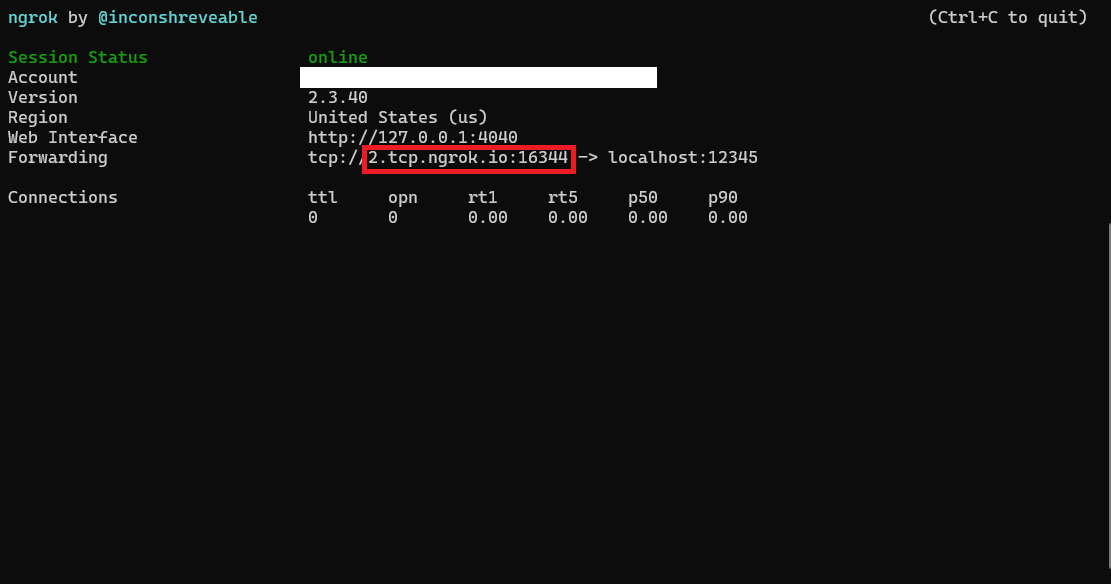
\includegraphics[width = 1.0 \textwidth]{images/2.png}
\end{center}

مهم‌ترین داده موجود در این صفحه، قسمتی است که در تصویر بالا دور آن کادر قرمز کشیده‌ شده است. برای این که بتوانید از بیرون (یک کامپیوتر دیگر) به سرور خود متصل شوید، لازم است که به جای آی‌پی محلی \lr{127.0.0.1}  که تا به حال به آن درخواست می‌زنید به این آدرس درخواست بزنید. یعنی در کلاینت شما، باید این آدرس را جایگزین کنید. به عنوان مثال، در مورد بالا باید سوکت سمت کلاینت شما به این شکل ساخته بشود:


\begin{latin}
\begin{lstlisting}[language = java]
socket = new Socket("2.tcp.ngrok.io", 16344);
\end{lstlisting}
\end{latin}

با این کار به راحتی امکان ارتباط برقرار کردن با سرور خود را از بیرون خواهید داشت.


\textbf{
	در کل تمام کاری که شما باید انجام بدهید، ساخت اکانت در \lr{ngrok}، اجرای درست \lr{ngrok} و تنظیم آدرس سوکت سمت کلاینت متناسب با آدرس داده شده در \lr{ngrok} است و نیازی به هیچ تغییر دیگری در کدهای خود نخواهید داشت.}





\end{document}
